\chapter{Fluid Dynamics and Bernoulli's Equation}

\section{Definitions}
\paragraph{Streamline (SL)}
Streamlines are lines that are tangent to the velocity vector field at all points in space.

\begin{figure}[H]
	\centering
	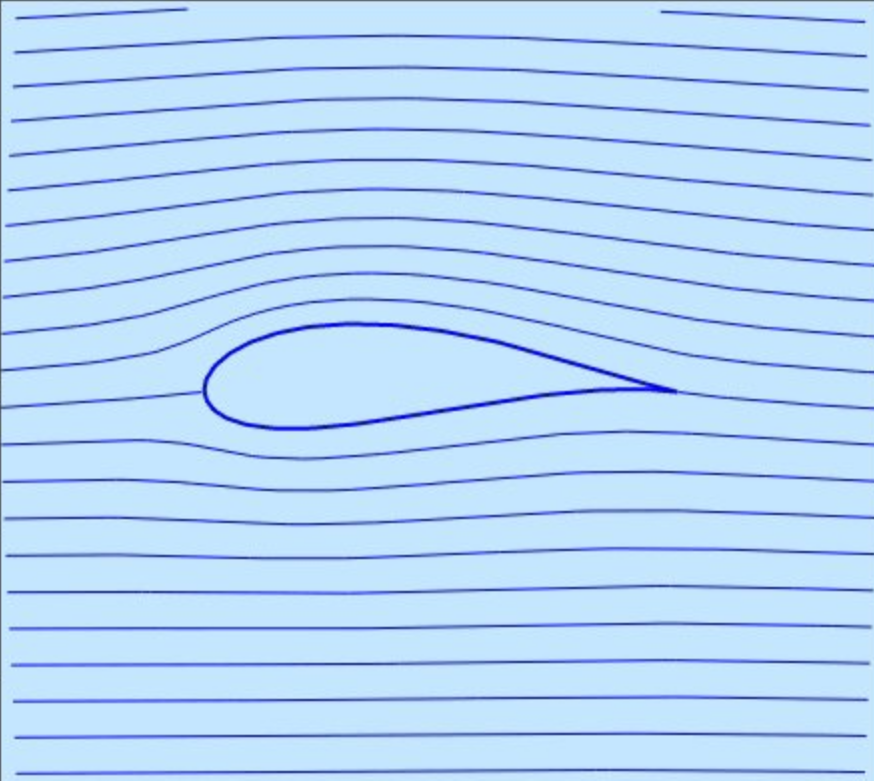
\includegraphics[width=0.3\linewidth]{Sketches/Airfoil}
	\caption{Streamlines along an airfoil}
	\label{fig:airfoil}
\end{figure}

\paragraph{Steady Flow}
When the velocity field $\vec v(\vec r, t)$ is time independent, we call the flow field \textbf{steady}. In this case the stream line is followed by fluid elements.


\section{Derivation of Bernoulli's Equation}

Recall newtons second law per unit volume \eqref{eq:newtons_second_law_per_unit_volume}:
\begin{equation*}
	-\nabla p - \rho g \hat k = \rho \vec a.
\end{equation*}

\begin{figure}[H]
	\centering
	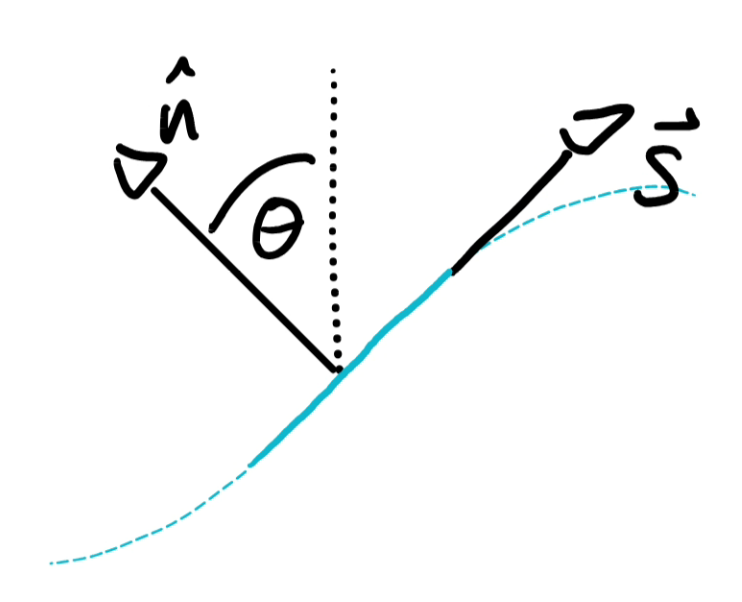
\includegraphics[width=0.3\linewidth]{Sketches/AlongStreamline}
	\caption{Coordinate system setup along a streamline.}
	\label{fig:alongstreamline}
\end{figure}

Along a stream line, (\ref{fig:alongstreamline}) with a normal with an angle $\theta$ to the vertical, we can use \eqref{eq:newtons_second_law_per_unit_volume} to state:


\begin{equation*}
	\begin{split}
		\vec a &= \frac{d\vec v}{dt} = a_s \hat s + a_n \hat n\\
		\text{in s-direction:}\quad a_s &= \frac{\partial v}{\partial s} \frac{\partial s}{\partial t} = \frac{\partial v}{\partial s} v\\
		\implies -\frac{\partial p}{\partial s} - \rho g\sin\theta &= \rho v\frac{\partial v}{\partial s}\\
		-\frac{\partial p}{\partial s} - \rho g \frac{\partial z}{\partial s} &= \rho \frac 12 \frac{\partial (v^2)}{\partial s}\\
		\frac 12 \rho \frac{\partial (v^2)}{\partial s} + \frac{\partial p}{\partial s} + \rho g \frac{\partial s}{\partial s} &= 0
	\end{split}
\end{equation*}

We integrate this along the streamline (in $s$), under the assumption that $\rho$ is constant:
\begin{equation*}
	\boxed{\frac 12 \rho v^2 + p + \rho g z = C}
	\label{eq:bernoullis_equation}
\end{equation*}
Which is \textbf{Bernoulli's Equation}, with units of energy per unit volume, or pressure. This equation is only valid if:
\begin{itemize}
	\item we have steady flow
	\item $\rho$ is constant
	\item we calculate along one streamline
	\item we can neglect viscosity / we have no shear forces.
\end{itemize}

Its first component ($v^2p/2$) is called \textbf{dynamic pressure}, the second ($p$) is the \textbf{static pressure}, the third ($\rho gz$) is called \textbf{head pressure} or \textbf{elevation pressure}. The first and second term combined is the \textbf{stagnation pressure}

\subsection{Stagnation Streamline}

\begin{figure}[H]
	\centering
	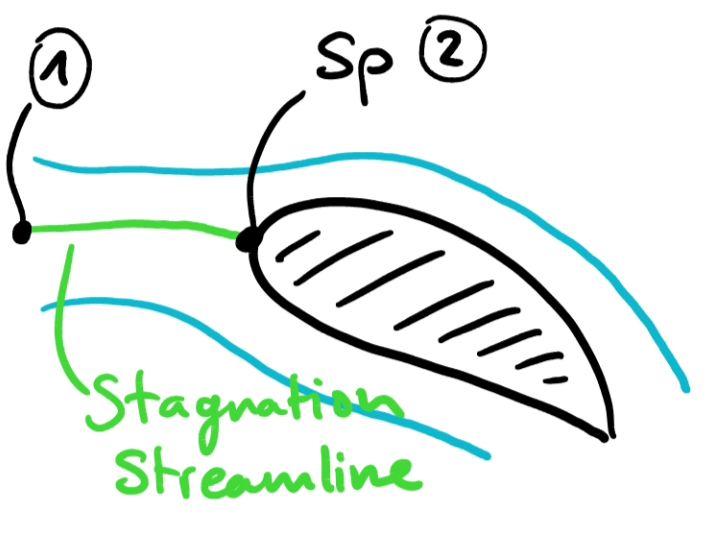
\includegraphics[width=0.3\linewidth]{Sketches/StagnationStreamline}
	\caption{The centred streamline that ends in the \textbf{Stagnation Point} (SP) is called \textbf{Stagnation Streamline}.}
	\label{fig:stagnationstreamline}
\end{figure}
Applying the Bernoulli's Equation for the stagnation streamline, yields:
\begin{equation*}
	p_1+\frac 12\rho v_1^2 = p_2 + \frac 12 \cancel{\rho v_2^2}^{\ast}
\end{equation*}
We ignored the $z$ term, because the pressure differences at flying altitude are negligible compared to the velocity of a plane. We cancel $\ast$ by the observation, that the velocity of the stream at the stagnation point is zero.

\subsection{Newton's 2nd law Across Streamlines}

Recall the coordinate system setup along a streamline (\ref{fig:alongstreamline}). To derive Bernoulli's Equation, we looked in the $s$-direction. If we look in the streamline-normal direction $\hat n$, we arrive at:
\begin{equation*}
	\begin{split}
		-\frac{\partial p}{n}-\rho g \cos \theta &= \rho \frac {v^2}R\qquad \left| \cos \theta= \frac{\partial z}{\partial n}\right.\\
		-\frac {dp}{dn}-\rho g \frac{dz}{dn} = \rho \frac{v^2}R\\
		-dp - \rho g \,dz &= \rho \frac{v^2}R dn
	\end{split}
\end{equation*}
Where $R$ is the \textbf{radius of curvature along $\hat n$}. We integrate the above term across the streamline, in $\hat n$ direction, yielding an important result:
\begin{equation}
		 \boxed{p + \rho gz + \rho \int \frac{v^2}{R}\,dn = C}
\end{equation}
Not knowing $R$ in the most cases makes this result unusable. However, if we have rectilinear (or nearly rectilinear) streamlines, the integration term disappears, as $R \to \infty$. From this we get the much more useable form:
\begin{equation}
	\boxed{p + \rho gz = C}
\end{equation}
\begin{figure}[H]
	\centering
	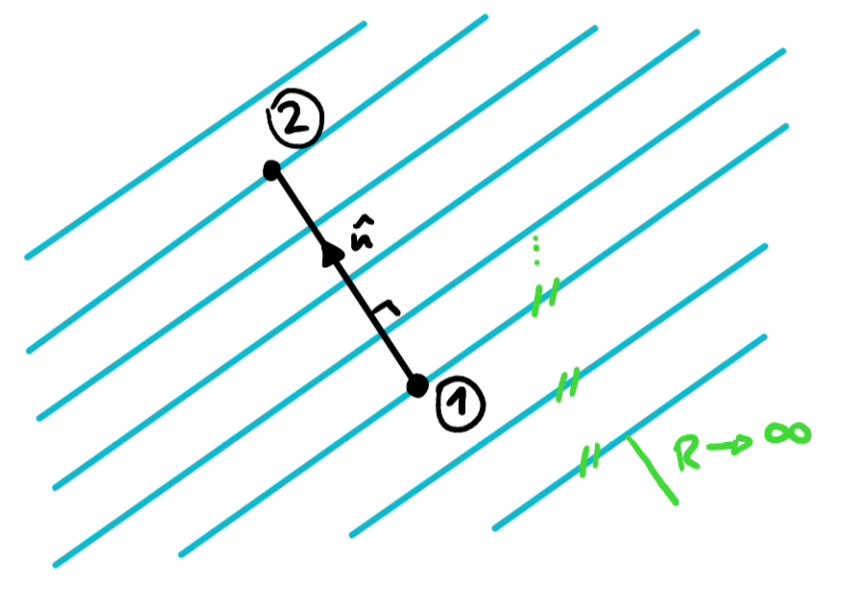
\includegraphics[width=0.4\linewidth]{Sketches/RectilinearStreamLines}
	\caption{All the streamlines are parallel to each other and straight ($R\to \infty$). We can take the difference between two points along the perpendicular direction $\hat n$.}
	\label{fig:rectilinearstreamlines}
\end{figure}
Applying this to a case like \ref{fig:rectilinearstreamlines} yields:
\begin{equation}
	p_2-p_1 = -\rho g (z_2-z_1) \implies p_1 = p_2+\rho gh
\end{equation}
Which can be recognized as one of the laws from hydrostatics.